\documentclass[border=3pt]{standalone}
% Preâmbulo compartilhado pelos diagramas TikZ da aula 13 (SLAM com EKF)
\usepackage[T1]{fontenc}
\usepackage[utf8]{inputenc}
\usepackage{lmodern}
\usepackage{amsmath}
\usepackage{xcolor}
\usepackage{tikz}
\usetikzlibrary{arrows.meta,angles,quotes,decorations.pathmorphing,decorations.pathreplacing,calc,
                positioning,shapes.geometric,shapes.misc,backgrounds,fit,
                math}

% Paleta (mesma dos SVGs originais)
\definecolor{dblue}{HTML}{2A5B8C}
\definecolor{dorange}{HTML}{B3541E}
\definecolor{dgreen}{HTML}{4A7C59}
\definecolor{dred}{HTML}{9C4B4B}
\definecolor{dcream}{HTML}{F4F1EA}
\definecolor{dshade}{HTML}{DDD7C9}

% Função gaussiana (não normalizada por padrão de escala visual)
\pgfmathdeclarefunction{gauss}{3}{%
  \pgfmathparse{1/(#3*sqrt(2*pi))*exp(-((#1-#2)^2)/(2*#3^2))}%
}

% Estilos comuns (prefixo d... para não colidir com chaves internas do pgf)
\tikzset{
  >={Stealth[length=2mm]},
  dguide/.style={gray!55, dashed, line width=0.4pt},
  daxis/.style={gray!60, line width=0.7pt, ->},
  dbody/.style={fill=black!3, draw=black!80, line width=1pt},
  dacc/.style={draw=dblue, line width=1pt},
  dlbl/.style={black!55, font=\small},
  dsub/.style={black!45, font=\footnotesize},
  dstate/.style={circle, draw=black!80, fill=dcream, line width=1pt,
                 minimum size=17mm, font=\large, inner sep=1pt},
  dobs/.style={circle, draw=black!80, fill=dshade, line width=1pt,
               minimum size=14mm, font=\large, inner sep=1pt},
  dbox/.style={rounded corners=2pt, draw=black!80, fill=dcream, line width=1pt,
               align=center, inner sep=6pt},
  dop/.style={circle, draw=black!80, fill=white, line width=1pt,
              minimum size=6mm, inner sep=0pt, font=\small},
  dtrans/.style={->, dblue, line width=1pt},
  dmeas/.style={->, dorange, line width=1pt},
  dcurve/.style={line width=1pt, dblue},
  dcurveb/.style={line width=1.4pt, dorange},
}

\begin{document}
\hyphenpenalty=10000 \exhyphenpenalty=10000 \tolerance=9999 \emergencystretch=3em
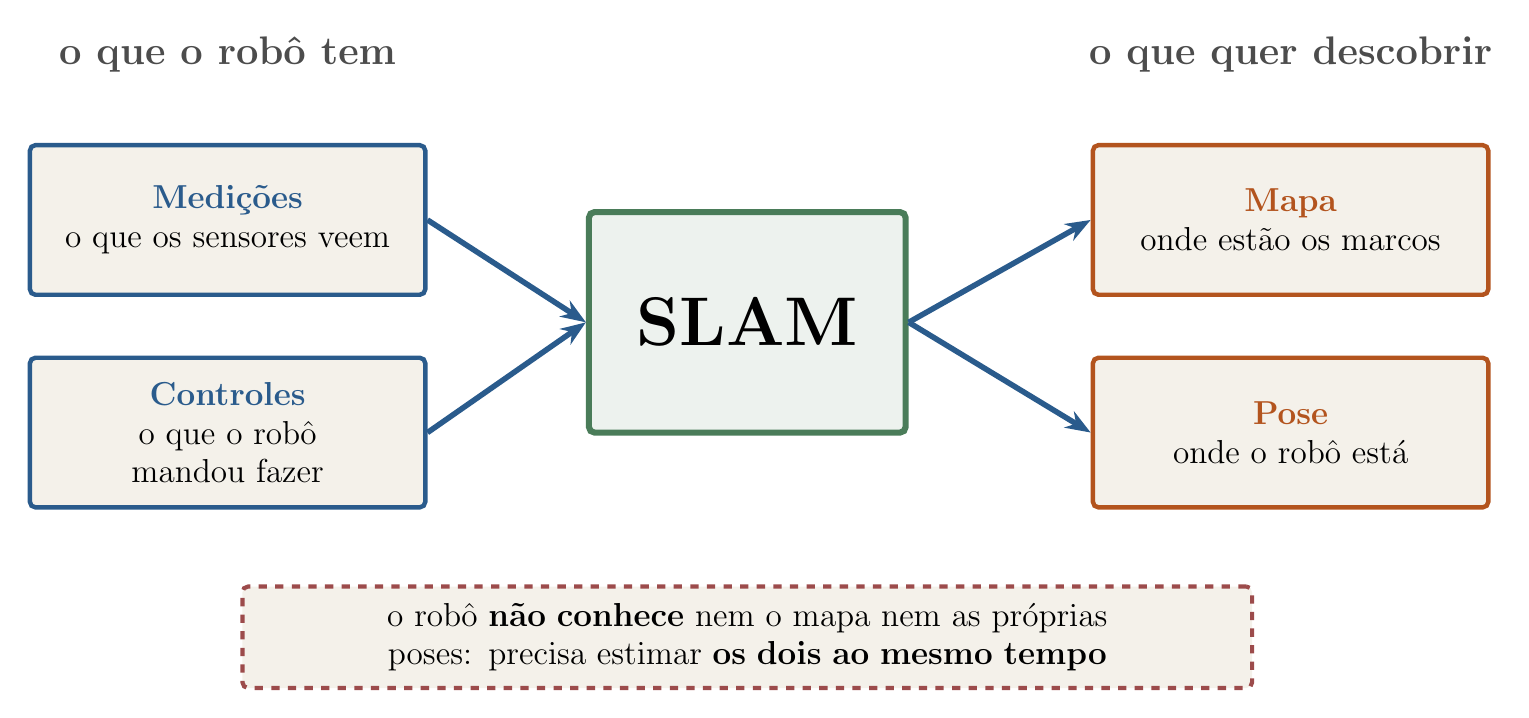
\begin{tikzpicture}[x=1cm,y=1cm]
\tikzset{c/.style={dbox, text width=4.6cm, minimum height=1.9cm, font=\large, line width=1.6pt}}
\node[font=\Large\bfseries, black!70] at (2.9,8.3) {o que o robô tem};
\node[font=\Large\bfseries, black!70] at (16.4,8.3) {o que quer descobrir};
\node[c, draw=dblue] (a) at (2.9,6.2) {\textbf{\textcolor{dblue}{Medições}}\\ o que os sensores veem};
\node[c, draw=dblue] (b) at (2.9,3.5) {\textbf{\textcolor{dblue}{Controles}}\\ o que o robô mandou fazer};
\node[dbox, draw=dgreen, fill=dgreen!10, line width=2.2pt, text width=3.6cm, minimum height=2.8cm, font=\Huge\bfseries] (s) at (9.5,4.9) {SLAM};
\node[c, draw=dorange] (m) at (16.4,6.2) {\textbf{\textcolor{dorange}{Mapa}}\\ onde estão os marcos};
\node[c, draw=dorange] (p) at (16.4,3.5) {\textbf{\textcolor{dorange}{Pose}}\\ onde o robô está};
\foreach \n in {a,b} {\draw[dtrans, line width=2pt, -{Stealth[length=3.2mm]}] (\n.east) -- (s.west);}
\foreach \n in {m,p} {\draw[dtrans, line width=2pt, -{Stealth[length=3.2mm]}] (s.east) -- (\n.west);}
\node[dbox, draw=dred, dashed, line width=1.5pt, text width=12.4cm, minimum height=1.2cm, font=\large] at (9.5,0.9) {o robô \textbf{não conhece} nem o mapa nem as próprias poses: precisa estimar \textbf{os dois ao mesmo tempo}};
\end{tikzpicture}
\end{document}
